This chapter describes the seismic source typologies supported by the OQ-engine: \textit{Point} and
\textit{Area} sources for modeling distributed seismicity, \textit{Simple Fault}, \textit{Complex Fault}, and
\textit{Characteristic Fault} for modeling fault-based seismcity.

\section{Basic concepts}
The OQ-engine provides several seismic source typologies to accomodate different modeling approaches. For modeling distributed seismicity, that is seismic activity occurring over a geographilcal region and not tight to
specific well characterized fault structures, the OQ-engine provides the \textit{Point} and \textit{Area} sources.
The former defines seismic activity nucleating in a single geographical location, while the second seismicity occurring uniformly over a geographical region. A collection of Point sources can be used to model seismicity with spatially variable parameters (as obtained from a smoothed seismicity approach for instance), while Area
sources can be used to model seismicity in geographic zones usually defined by expert judgments
taking into account seismological, geological and geodetic information.\\
For modeling fault-based seismicity, that is seismic activity occurring on a well identified and characterized
fault zone, the OQ-engine provides two main options, the \textit{Simple Fault} and \textit{Complex Fault}
sources. Both source typologies allows modeling earthquakes on faults as \textit{floating ruptures}, that is as
portions of the fault surface which are moved (that is 'floated') over the entire fault surface to simulate all possible rupture locations. The two source typologies differs instead in terms of the geometrical complexity
they can accomodate when modeling a fault surface. In particular, a Simple Fault source can model a fault
surface as a plain rectangle in the simplest case, or a set of connected parallelograms in the most complex
case. A Complex Fault source can instead model an arbitrarily complex quadrilateral surface, which can
therefore accomodate changes in dip angle along depth or along strike or changes in fault width. The
Complex Fault source is therefore particularly suitable for modeling large subdution interface surfaces, while
Simple Fault sources can be used for modeling crustal faults. The \textit{Characteristic Fault} source can model both simple and complex geometries, but instead of simulating floating ruptures, each earthquake
rupture the entire fault surface indipendently of the associated magnitude. The Characteristic Source typology
can be used to model individual faults or fault segments that tend to produce essentialy same size
earthquakes (CITE SCHWARTZ COPPERSMITH 1984).\\
\section{The Point and Area sources}
The parameters required for the definition of Point and Area sources, and their associated function, are listed in Table \ref{table:point_area_tab}.
\begin{table}
\caption{Table summarizing parameters, and their functions, required for the definition of Area and Point
sources in the OQ-engine}
\centering
\begin{tabular}{p{60mm} p{60mm}}
\specialrule{.2em}{.1em}{.4em} 
Parameter & Purpose \\ [0.5ex] % inserts table
\specialrule{.2em}{.1em}{.4em}
Magnitude frequency distribution & Defines total moment rate of a source\\ 
\specialrule{.05em}{.1em}{.4em}
Magnitude area scaling relationship & Define sizes and shapes of rupture planes \\
Rupture aspect ratio (length / width) & \\
\specialrule{.05em}{.1em}{.4em}
Nodal plane distribution \newline (each nodal plane being defined \newline by strike, dip, rake) & Defines orientations and faulting styles of ruptures \\
\specialrule{.05em}{.1em}{.4em}
Hypocentral depth distribution &  Defines centroids of rupture planes \\
\specialrule{.05em}{.1em}{.4em}
Upper seismogenic depth & Constrains rupture planes inside seismogenic layer \\
Lower seismogenic depth & \\
\hline %inserts single line
\end{tabular}
\label{table:point_area_tab}
\end{table}
Sources are parameterized so that earthquake ruptures are modeled as planar rectangles in a 3D space. In a point-source representation (Figure \ref{fig:PointSource}) ruptures are generated underneath a single geographical location, and can be potentially distributed over multiple orientations, faulting styles, and depth levels.
\begin{figure}
\centering
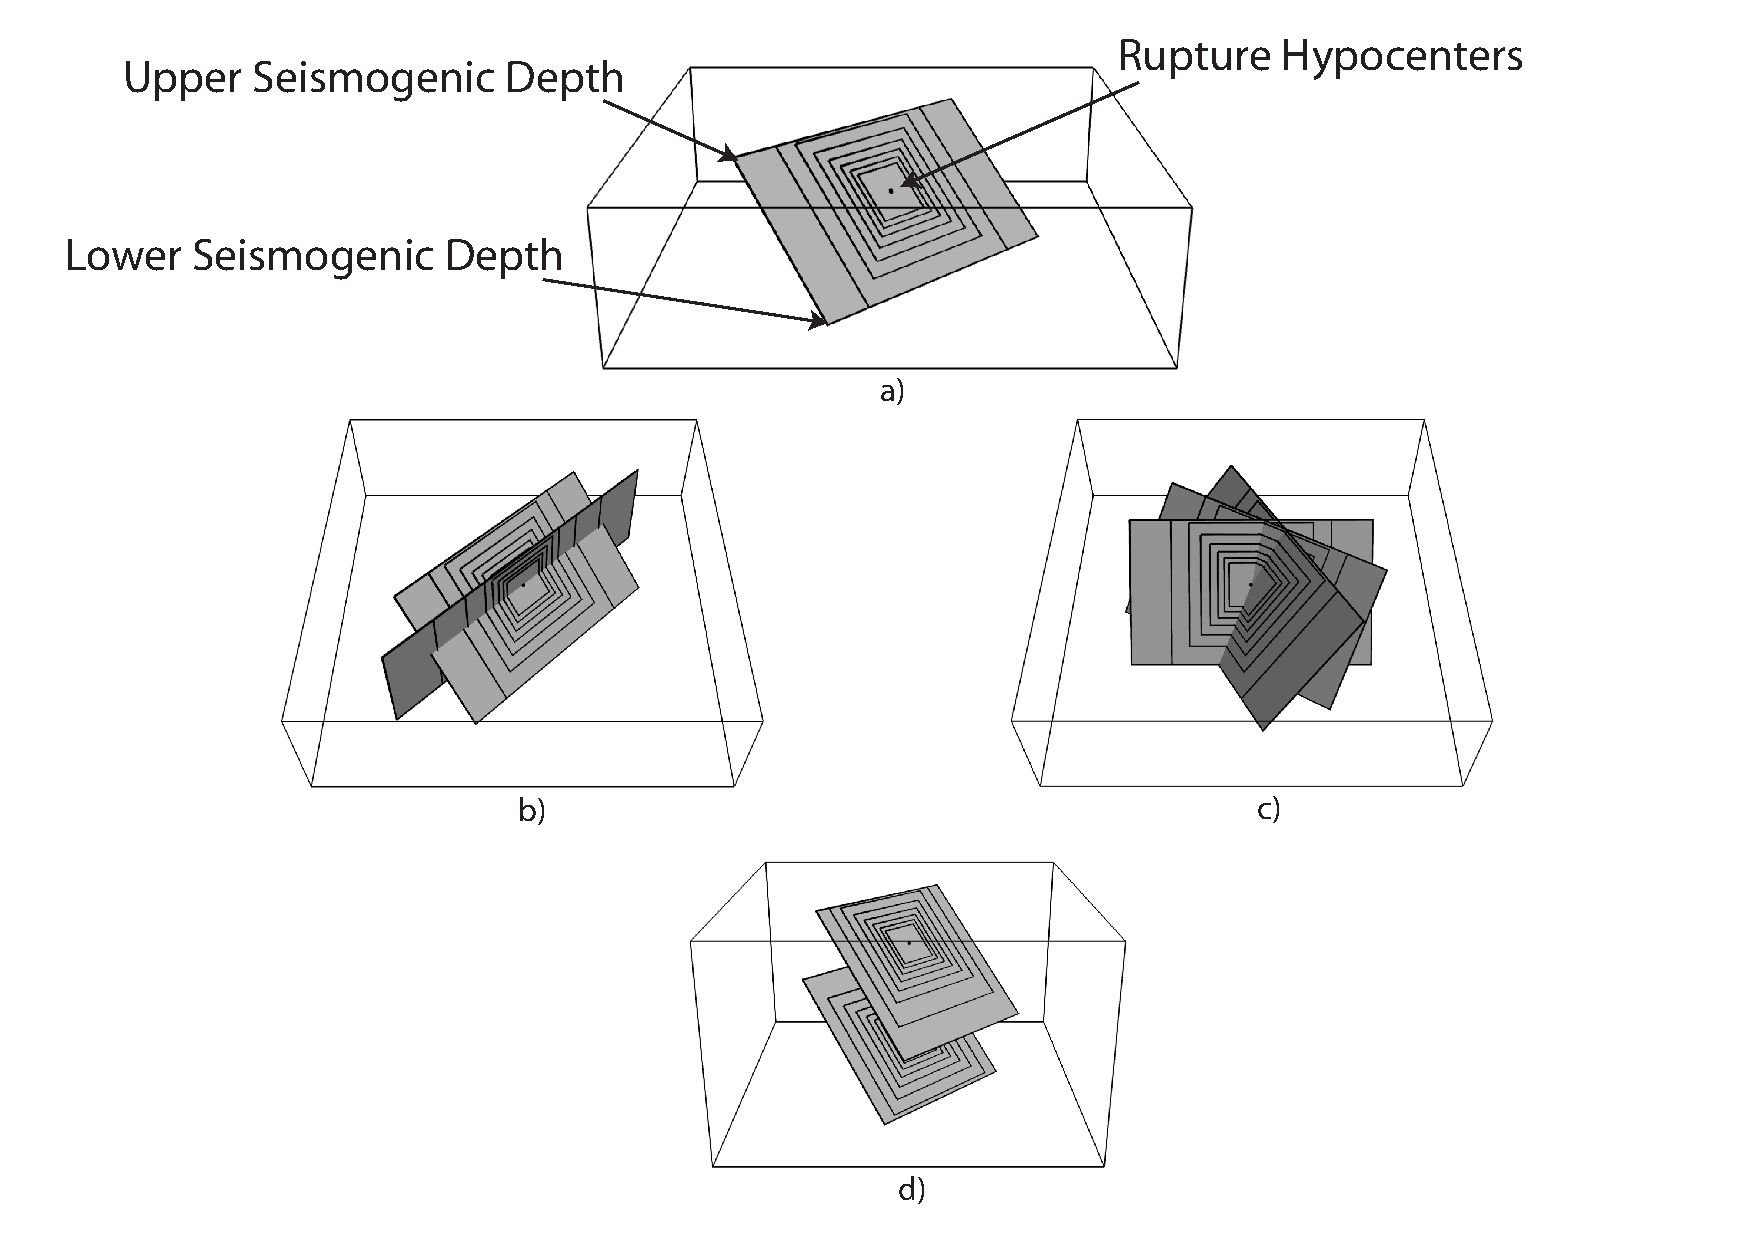
\includegraphics[width=14cm]{./Pictures/PointSource.pdf}
\caption{Graphical representation of the earthquake ruptures as generated by a Point Source. a) Given a geographical location on the earth surface, ruptures are generated underneath according to a scaling relationship and aspect ratio value and forced to not exceed the upper and lower seismogenic depths. Ruptures can be distributed over multiple dips b), strikes c) and hypocentral depths d).}
\label{fig:PointSource}
\end{figure}
Rupture centroids are co-located with the point-source location and are positioned at depths specified by the hypocentral depth distribution. Rupture shapes follow the given aspect ratio. However, if for a given aspect ratio and hypocentral depth the rupture plane crosses either boundary (upper or lower) of the seismogenic layer, the plane is shifted along the dip direction so as to fit within the upper and lower seismogenic depths. As a consequence, the hypocentral location no longer corresponds with the plane centroid. If this adjustment is insufficient to avoid crossing either boundary of the seismogenic layer, the plane is reshaped; the width becomes the maximum allowed by the seismogenic layer thickness, and the length is increased so as to conserve rupture area (at the expense of the aspect ratio).\\
In an area source (Figure \ref{fig:AreaSource}), earthquake ruptures are distributed over a regular grid (equally-spaced in distance) covering a geographical region as defined by a seismic zone. 
\begin{figure}
\centering
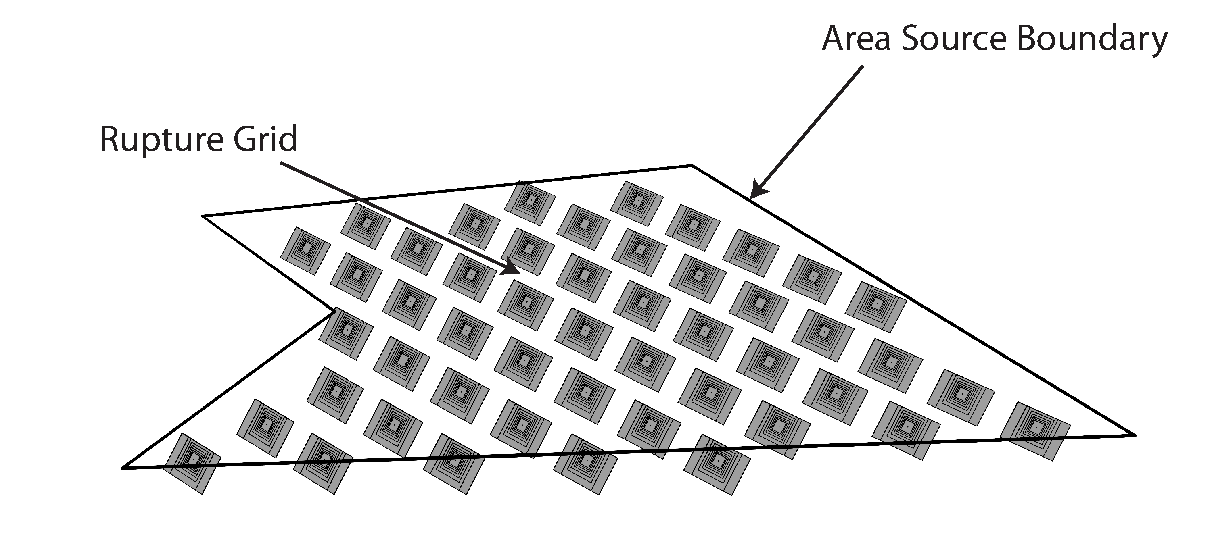
\includegraphics[width=14cm]{./Pictures/AreaSource.pdf}
\caption{Earthquake ruptures generated by an area source in the OQ-engine. Ruptures are distributed uniformly over a regular grid within the area. In this plot, for better visualization, ruptures are modeled only according to a single nodal plane and hypocentral depth, but actual calculations may involve multiple orientations and hypocentral depths. Ruptures originating from different grid nodes may also overlap and cross each other.}
\label{fig:AreaSource}
\end{figure}
Generation of ruptures follows the same algorithm as for point sources. For both sources, the rate associated to each rupture plane is the original rate associated to the corresponding magnitude bin, scaled by the location weight (1 for a point source and 1 / N for an area source, where N is the total number of grid points in the area), the nodal plane (that is orientation and faulting style) weight, and the hypocentral depth weight.\\
For an area source, the boundary is assumed ‘leaky’, that is earthquake ruptures can extend out of it. Because of rupture area conservation, earthquake surfaces associated to large magnitudes can extend well beyond the source boundaries. If the rupture orientation is considered random then this behavior can potentially lead to unrealistic scenarios, that is earthquake ruptures that are not consistent with the area geometry and the tectonic feature it is meant to represent. The design of an area source requires therefore a careful estimation not only of the associated activity rates but also of the predominant faulting orientations.\\
\section{The Simple Fault source}
Parameters required for the definition of a Simple Fault source are given in Table \ref{table:simple_fault_tab}.
\begin{table}
\caption{Table summarizing parameters, and their functions, required for the definition of a Simple Fault source in the OQ-engine}
\centering
\begin{tabular}{p{60mm} p{60mm}}
\specialrule{.2em}{.1em}{.4em} 
Parameter & Purpose \\ [0.5ex] % inserts table
\specialrule{.2em}{.1em}{.4em}
Magnitude frequency distribution & Defines total moment rate of a source\\ 
\specialrule{.05em}{.1em}{.4em}
Magnitude area scaling relationship & Define sizes and shapes of rupture planes \\
Rupture aspect ratio (length / width) & \\
\specialrule{.05em}{.1em}{.4em}
Fault trace & Define fault surface \\
Upper seismogenic depth & \\
Lower seismogenic depth & \\
Dip angle & \\
\specialrule{.05em}{.1em}{.4em}
Rake angle & Defines faulting style \\
\hline %inserts single line
\end{tabular}
\label{table:simple_fault_tab}
\end{table}
The fault surface is constructed by translating the fault trace from the upper to the lower seismogenic depth along a direction perpendicular to the fault trace (measured as the difference between the azimuths of the first and last coordinates of the trace) and with an inclination equal to the dip angle. The surface so defined is
effectively modeled as a regular (i.e. equally spaced in distance) mesh (Figure
\ref{fig:SimpleFaultSource_mesh}).
\begin{figure}
\centering
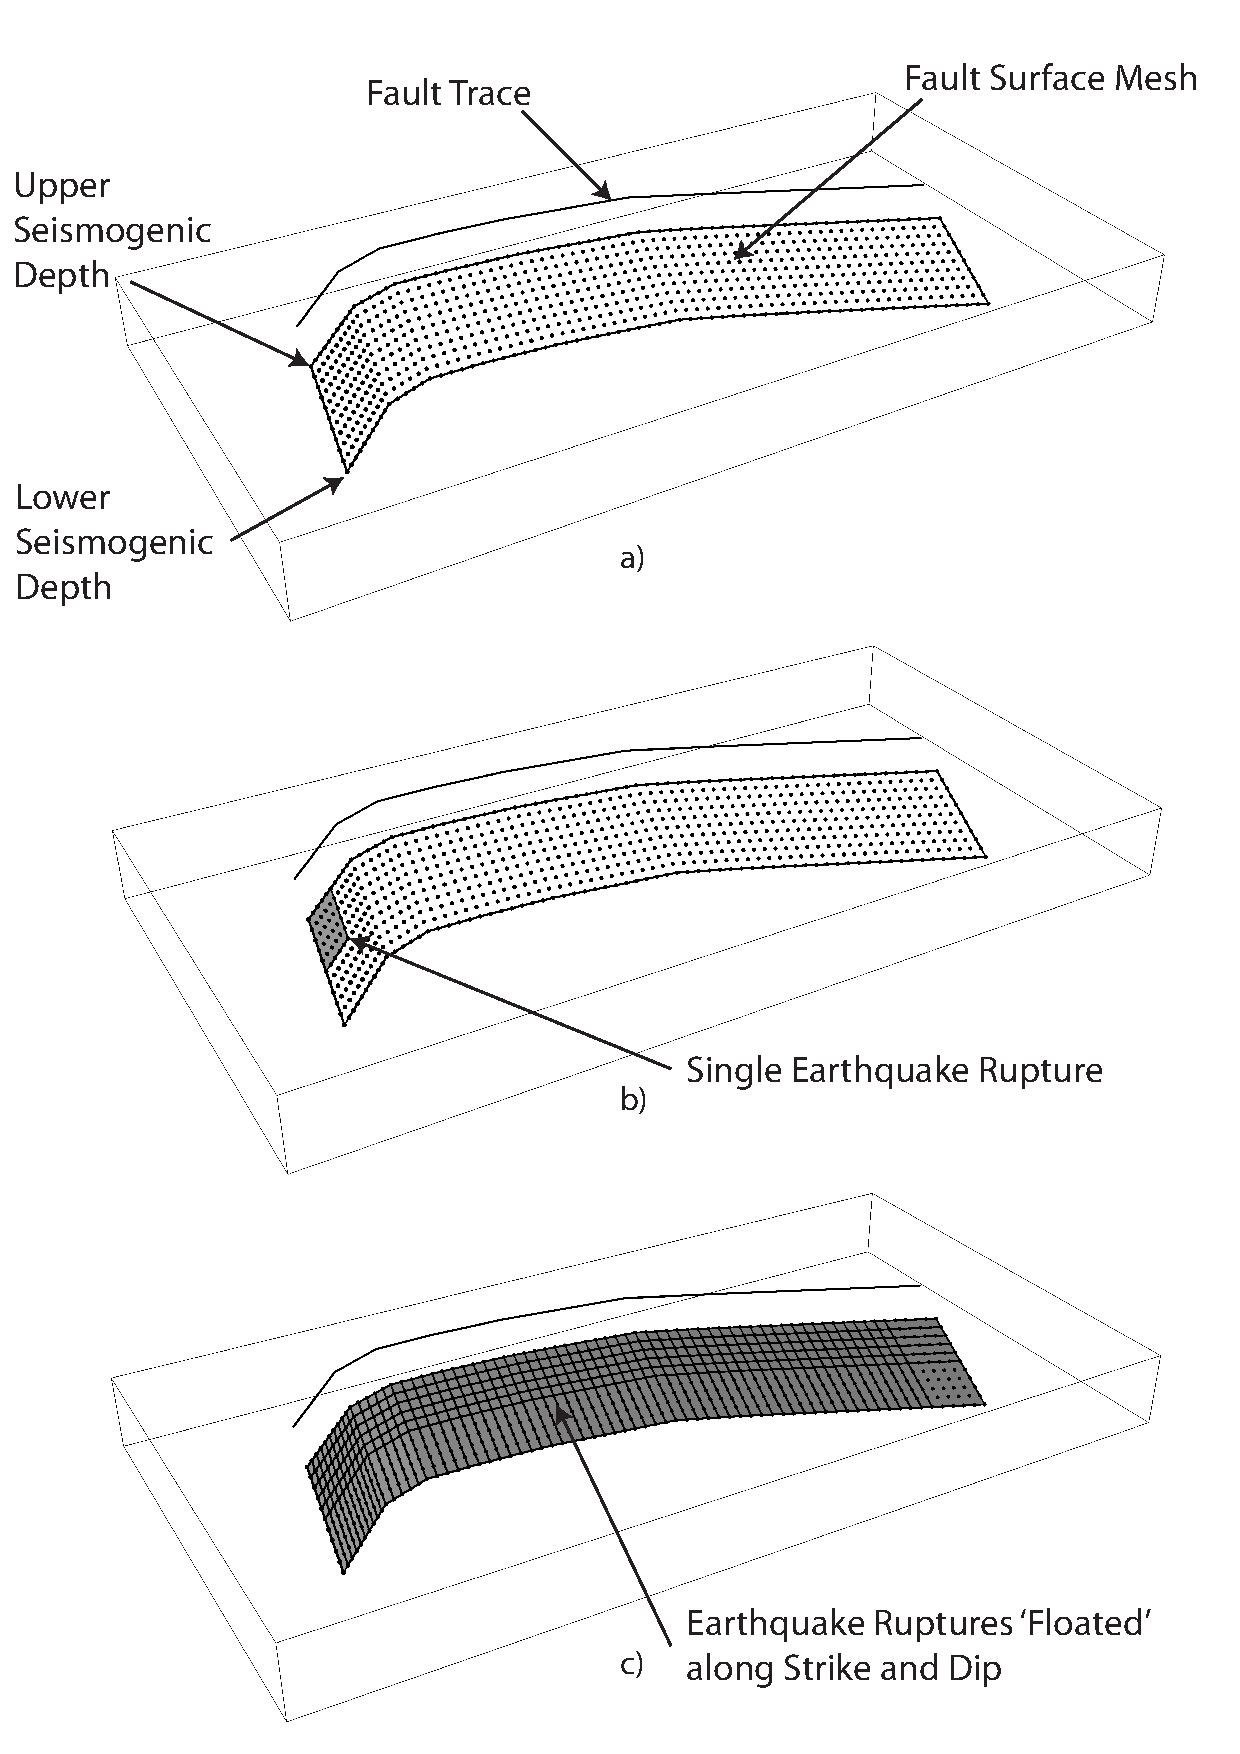
\includegraphics[width=14cm]{./Pictures/SimpleFaultSource.pdf}
\caption{Simple Fault source}
\label{fig:SimpleFaultSource}
\end{figure}
For each magnitude bin defined in the magnitude-frequency distribution, an earthquake rupture is modeled as a portion of the fault surface, accordingly with the magnitude scaling relationship and the rupture aspect
ratio. To simulate all possible rupture locations, each earthquake rupture is \textit{floated}, that is moved,
along both the strike and dip directions. The floating step is assumed equal to the mesh discretization step.
The occurrence rate associated to a given magnitude bin is distributed uniformly over all the ruptures associated with the same magnitude value. 
\ref{fig:SimpleFaultSource_mesh}).
\section{The Complex Fault source}
\begin{figure}
\centering
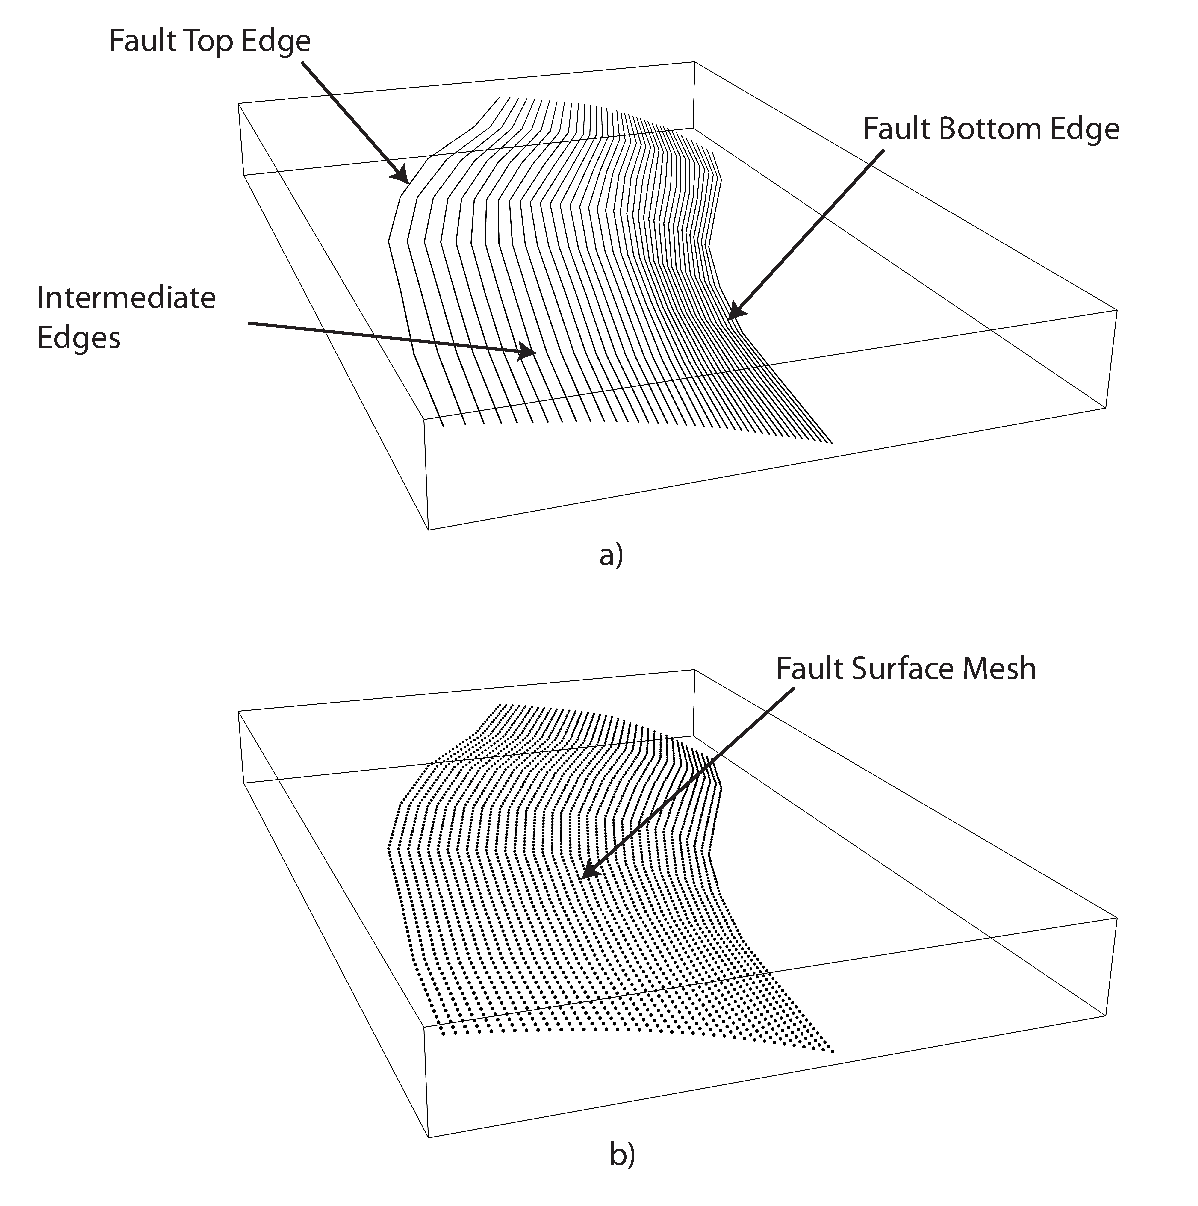
\includegraphics[width=14cm]{./Pictures/ComplexFault.pdf}
\caption{Complex Fault source}
\label{fig:ComplexFaultSource}
\end{figure}
%\begin{figure}
%\centering
%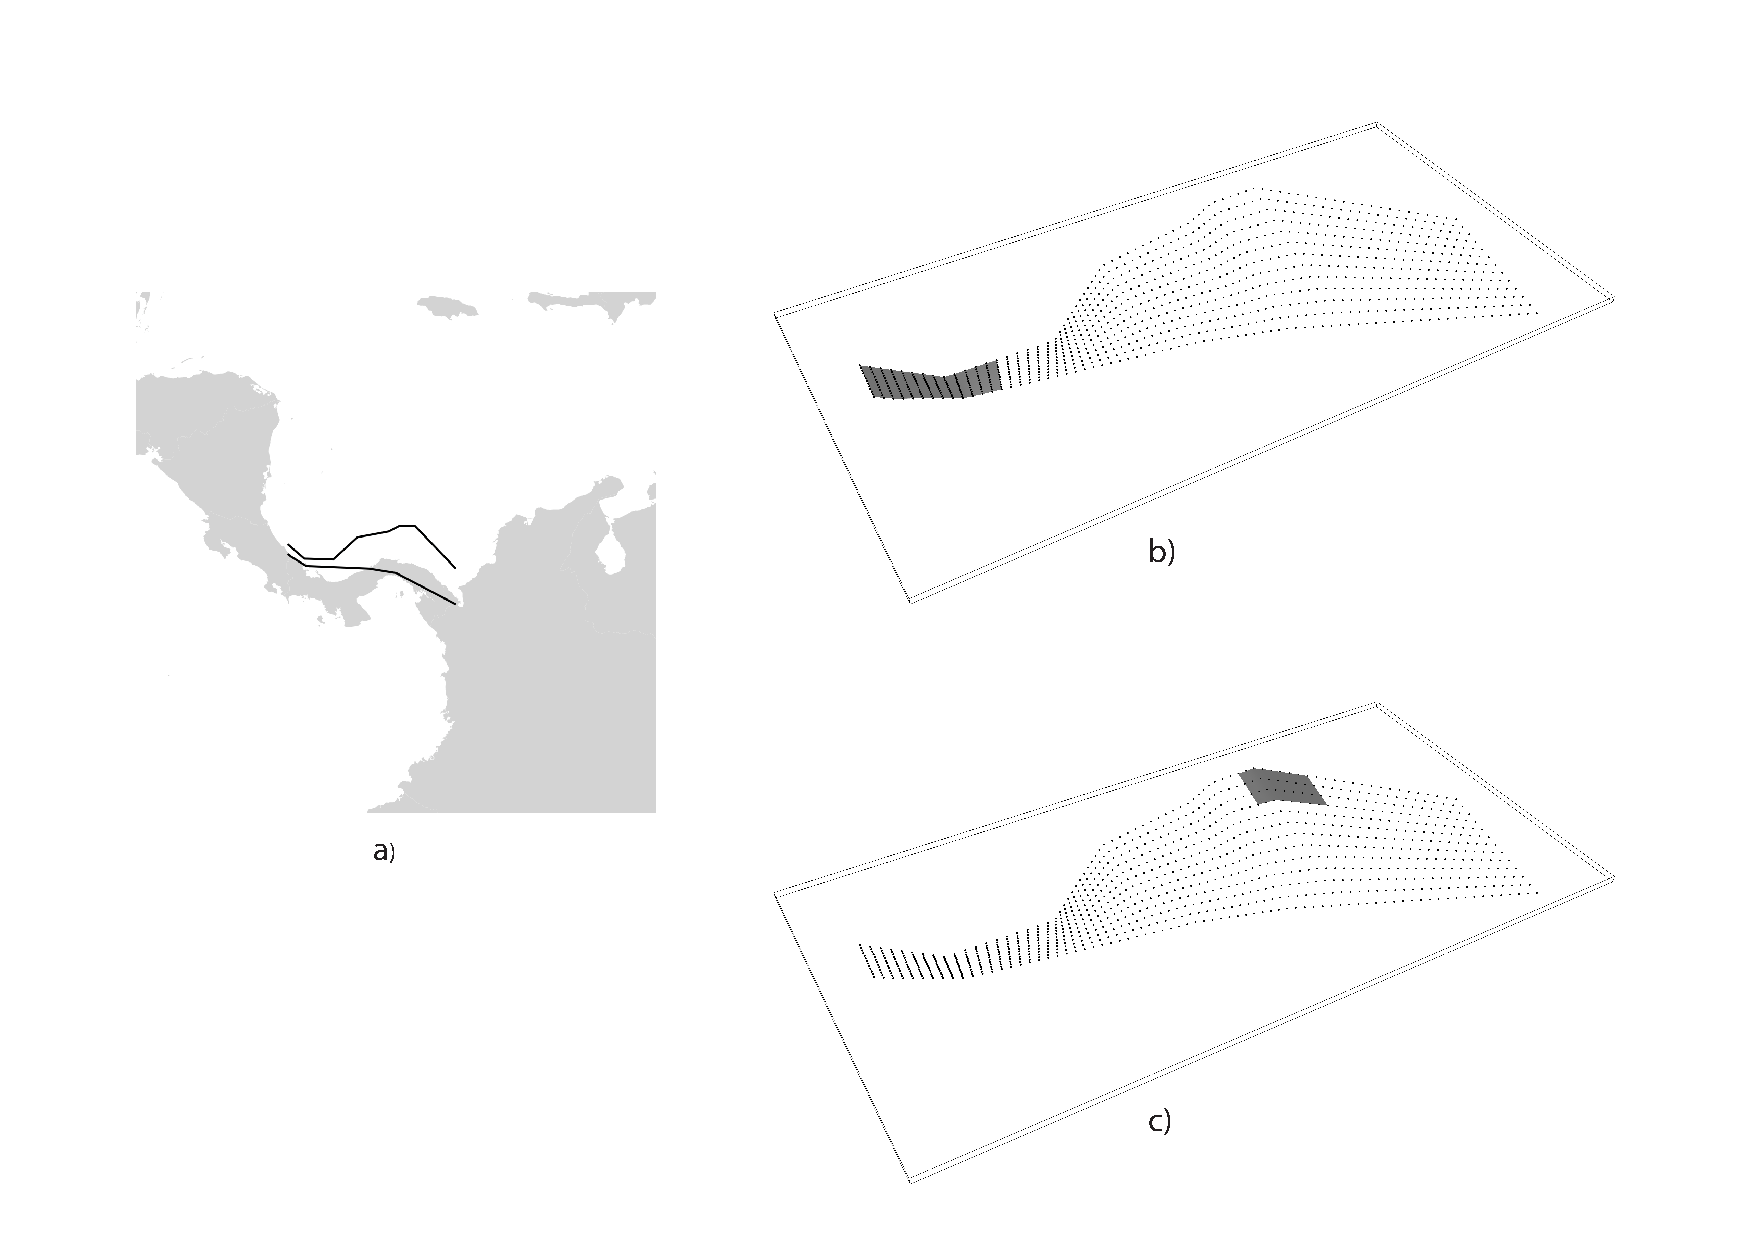
\includegraphics[width=14cm]{./Pictures/ComplexFaultPanama.jpg}
%\caption{Complex Fault source}
%\label{fig:ComplexFaultSourcePanama}
%\end{figure}
%\begin{figure}
%\centering
%\begin{center}
%\begin{array}{c}
%\includegraphics[width=14cm]{./Pictures/SimpleFaultSource_mag6_loc0.jpg}
%\includegraphics[width=14cm]{./Pictures/SimpleFaultSource_mag6_all_locs.jpg}
%\end{array}$
%\end{center}
%\caption{Example of earthquake rupture generated by a Simple Fault source.}
%\label{fig:SimpleFaultSource_mag6}
%\end{figure}
%
% ..............................................................................
%\section{Temporal occurrence model}
%\subsection{The Poisson model}
%\index{Temporal occurrence models!Poisson}
%
% ..............................................................................
%\section{Seismic sources for distributed seismicity modelling}
%\index{Distributed seismicity}
%
%Distributed seismicity is the seismicity can cannot be associated unambiguously
%to a specific fault structure.

%\subsection{The point source}
%\index{Seismic source!Point}
%
%\subsection{Area source}
%\index{Seismic source!Area}
%
% ..............................................................................
%\section{Fault sources}
%
%\subsection{Simple fault}
%\index{Seismic source!Simple fault}
%
%\subsection{Complex fault}
%\index{Seismic source!Complex fault}
%
%\subsection{Characteristic fault}
%\index{Seismic source!Characteristic fault}
%
%\section{Non-parametric sources}
%\index{Seismic source!Non-parametric}
